\documentclass[aspectratio=169]{beamer}
\usetheme{d2s}

% --- STANDARD & REQUIRED PACKAGES ---
\usepackage[T1]{fontenc}
\usepackage[export]{adjustbox}
\usepackage{upquote}
\usepackage{graphicx}
\usepackage{etoolbox}
\usepackage{listings}
\usepackage[most]{tcolorbox} % Use [most] to load all skins and features
\usepackage{tikz}
\usetikzlibrary{positioning, matrix, shapes.arrows, chains, decorations.pathreplacing}

% --- DOCUMENT INFORMATION ---
\title[Blockchain II — Day 5]{Day 5: Reaching Consensus}
\subtitle{Section II: Blockchain Fundamentals}
\author{Army Cyber Institute}
\institute{Army Cyber Institute, U.S. Military Academy}
\date{}

% --- BEAMER SETTINGS & CUSTOMIZATIONS ---
\setbeameroption{hide notes}


% --- HELPER COMMANDS & BOXES ---
\newcommand{\placeholdergraphic}[2][\linewidth]{%
  \begin{tcolorbox}[
    enhanced, colback=white, colframe=usmagray,
    title=Graphic placeholder, width=#1, sharp corners,
    boxrule=0.5pt, left=4pt,right=4pt,top=6pt,bottom=6pt
  ]
    \footnotesize #2
  \end{tcolorbox}
}

\newtcolorbox{keytermbox}[2][]{
  enhanced, colback=armygold!10, colframe=armygold!75!black,
  fonttitle=\bfseries, title=#2, rounded corners, halign title=left, #1
}


\begin{document}

% --- TITLE PAGE ---
\begin{frame}
    \titlepage
\end{frame}

% ---------------- SLIDE 0: Today's Roadmap ----------------
\begin{frame}{Today's Roadmap}
    \setbeamerfont{itemize}{size=\large}
    \begin{itemize}
        \item \textbf{Properties and Models}: SLVA, Faults, and Timing
        \item \textbf{Core Mechanics}: Quorums, Rounds, and Timeouts
        \item \textbf{Consensus Families}: CFT, BFT, and Nakamoto-Style
        \item \textbf{Application}: Trade-offs and a Bridge to PoW/PoS
    \end{itemize}
\end{frame}

% ========== SLIDE 1: Foundations of Consensus ==========
\begin{frame}{Foundations of Consensus}
\begin{columns}[T]
\begin{column}{0.6\linewidth}
    \begin{itemize}
        \item Formal guarantees for agreement in decentralized systems \cite{bano_blockchain_2017}.
        \item Property lens: \textbf{S}afety, \textbf{L}iveness, \textbf{V}alidity, \textbf{A}greement (SLVA).
        \item Today's path: Properties $\rightarrow$ Models $\rightarrow$ Mechanics $\rightarrow$ Families.
    \end{itemize}
    \vfill
    \begin{center}
    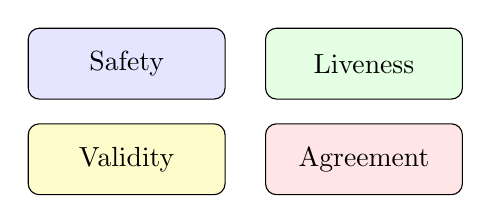
\begin{tikzpicture}[node distance=0.3cm and 0.5cm, prop/.style={draw, rounded corners, minimum width=2.5cm, minimum height=0.9cm, align=center}]
        \node[prop, fill=blue!10] (s) {Safety};
        \node[prop, fill=green!10, right=of s] (l) {Liveness};
        \node[prop, fill=yellow!20, below=of s] (v) {Validity};
        \node[prop, fill=red!10, below=of l] (a) {Agreement};
    \end{tikzpicture}
    \end{center}
\end{column}
\begin{column}{0.4\linewidth}
    \begin{tcolorbox}[colback=white,colframe=black!20,title=SLVA at a Glance]
    \small
    \begin{itemize}
      \item \textbf{Safety}: No conflicting commits \cite{porat_consensus_2017}.
      \item \textbf{Liveness}: Eventual progress \cite{porat_consensus_2017}.
      \item \textbf{Validity}: Only valid values decided.
      \item \textbf{Agreement}: Correct nodes converge.
    \end{itemize}
    \end{tcolorbox}
\end{column}
\end{columns}
\end{frame}

% ========== SLIDE 2: From Human Agreement to Algorithms ==========
\begin{frame}{From Human Agreement to Algorithms}
    \begin{itemize}
        \item Grounding complex algorithms in familiar human processes.
        \item Formalize models for faults (Crash/Byzantine) and timing (Sync/Async).
        \item Preview consensus families and their core trade-offs.
    \end{itemize}
    \vfill
    \begin{tcolorbox}[colback=white,colframe=black!20, title={Mapping Intuition to Protocol Mechanics}]
        \centering
        \large
        \renewcommand{\arraystretch}{1.5}
        \begin{tabular}{lcl}
            \textbf{Human Concept} & & \textbf{Digital Mechanism} \\
            \hline
            Jury / Supermajority Vote & $\rightarrow$ & Quorum (e.g., $2t+1$ votes) \cite{castro_practical_1999} \\
            Referee / Coordinator & $\rightarrow$ & Protocol Leader \\
            Shot Clock / Deadline & $\rightarrow$ & Timeout (triggers view change) \cite{10.1145/42282.42283}\\
        \end{tabular}
    \end{tcolorbox}
\end{frame}

% ========== SLIDE 3: Consensus Properties Defined ==========
\begin{frame}{Consensus Properties Defined}
    \begin{itemize}
        \item \textbf{Safety}: Nothing bad ever happens. Correct nodes \textit{never} decide conflicting values \cite{bano_blockchain_2017}.
        \item \textbf{Liveness}: Something good eventually happens. Correct nodes \textit{eventually} reach a decision \cite{bano_blockchain_2017}.
        \item \textbf{Validity}: The system respects application rules. Only \textit{admissible} values are decided.
        \item \textbf{Agreement}: Correct nodes that decide converge on the \textit{same} value.
    \end{itemize}
    \vfill 
    \begin{tcolorbox}[enhanced, colback=white, colframe=usmagray, title={Properties as Guarantees in Blockchains}]
    \small
    \begin{tabular}{lp{0.8\linewidth}}
         \textbf{Safety} & $\rightarrow$ Guarantees \textbf{Finality}. A finalized transaction will not be reversed. \\
         \textbf{Liveness} & $\rightarrow$ Guarantees \textbf{Progress}. The chain continues to grow. \\
         \textbf{Validity} & $\rightarrow$ Guarantees \textbf{Integrity}. Only valid blocks can be finalized. \\
         \textbf{Agreement} & $\rightarrow$ Guarantees \textbf{Consistency}. All honest nodes see the same ledger. \\
    \end{tabular}
    \end{tcolorbox}
\end{frame}

% ========== SLIDE 4: Failure and Timing Models ==========
\begin{frame}{Failure and Timing Models}
    \begin{tcolorbox}[enhanced, colback=d2s.fg!30, colframe=black, fonttitle=\bfseries, title={Fault and Timing Models}]
        \begin{columns}[T]
            \begin{column}{0.48\linewidth}
                \textbf{Fault Models}
                \begin{itemize}
                    \item \textbf{Crash}: Nodes stop, but don't lie.
                    \item \textbf{Byzantine}: Nodes can be malicious, lie, and collude \cite{lamport_byzantine_1982}.
                \end{itemize}
            \end{column}
            \begin{column}{0.52\linewidth}
                \textbf{Timing Models}
                \begin{itemize}
                    \item \textbf{Asynchronous}: Unbounded delay.
                    \item \textbf{Partially Synchronous}: Eventually bounded delay \cite{10.1145/42282.42283}.
                    \item \textbf{Synchronous}: Known, bounded delay.
                \end{itemize}
            \end{column}
        \end{columns}
    \end{tcolorbox}
    \vfill
    \begin{tcolorbox}[enhanced, colback=red!20, colframe=red!75!black, fonttitle=\bfseries, title={Landmark: FLP Impossibility}, rounded corners, drop shadow, valign=center]
    \small In a purely async network, no deterministic protocol can guarantee liveness if even one fault occurs \cite{fischer_impossibility_1985}. This necessitates the partially synchronous model for practical systems.
    \end{tcolorbox}
\end{frame}

% ========== SLIDE 5: Core Mechanics: Quorums, Rounds, and Timeouts ==========
\begin{frame}{Core Mechanics: Quorums, Rounds, and Timeouts}
    \begin{itemize}
        \item \textbf{Quorums}: Supermajority vote sets (e.g., $2t+1$) for safety through overlap \cite{castro_practical_1999}.
        \item \textbf{Rounds \& Phases}: Structures execution (propose, vote, commit) for auditability.
        \item \textbf{Timeouts}: Detects stalls and triggers leader rotation for liveness.
    \end{itemize}
    \vfill
    \begin{tcolorbox}[colback=white, colframe=usmagray, title={Anatomy of a BFT Round (Simplified)}]
        \centering
        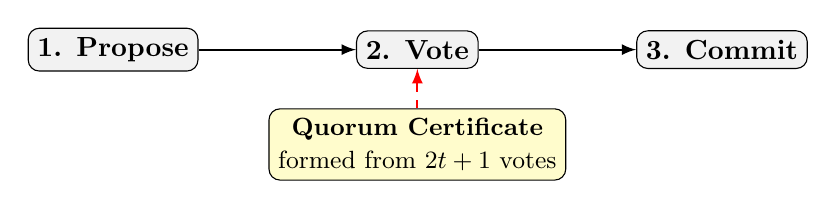
\begin{tikzpicture}
            \node[draw, rounded corners, fill=gray!10, font=\bfseries] (p) {1. Propose};
            \node[draw, rounded corners, fill=gray!10, font=\bfseries, right=2cm of p] (v) {2. Vote};
            \node[draw, rounded corners, fill=gray!10, font=\bfseries, right=2cm of v] (c) {3. Commit};
            \node[draw, fill=yellow!20, rounded corners, align=center, below=0.5cm of v] (qc) {\small \textbf{Quorum Certificate}\\\small formed from $2t+1$ votes};
            \draw[-latex, thick] (p) -- (v);
            \draw[-latex, thick] (v) -- (c);
            \draw[-latex, thick, red, dashed] (qc) -- (v);
        \end{tikzpicture}
    \end{tcolorbox}
\end{frame}

% ========== SLIDE 6: Comparing Consensus Families ==========
\begin{frame}{Comparing Consensus Families}
    \begin{itemize}
        \item \textbf{CFT (e.g., Raft):} For trusted clusters. Assumes only crash faults. Provides deterministic finality with low latency and energy use \cite{184040}.
        \item \textbf{BFT (e.g., PBFT):} For governed consortiums. Tolerates malicious (Byzantine) nodes. Provides deterministic finality with low-to-medium latency \cite{castro_practical_1999}.
        \item \textbf{Nakamoto (e.g., PoW):} For public networks. Open membership protected by economic costs (Sybil resistance). Finality is probabilistic and latency is high \cite{nakamoto_bitcoin_2008}.
    \end{itemize}
    \vfill
    \begin{tcolorbox}[enhanced, colback=red!20, colframe=red!75!black, fonttitle=\bfseries, title={Key Takeaway}, rounded corners, drop shadow]
    There is no "best" consensus algorithm \cite{bano_blockchain_2017}. The choice is a trade-off between permissioning, performance, and security assumptions, driven by the use case.
    \end{tcolorbox}
\end{frame}

% ========== SLIDE 7: Why Consensus Matters in Blockchains ==========
\begin{frame}{Why Consensus Matters in Blockchains}
    \begin{columns}[T]
        \begin{column}{0.5\linewidth}
            \begin{itemize}
                \item Solves the \textbf{double-spend problem} by creating one canonical history \cite{nakamoto_bitcoin_2008}.
                \item Replaces a central operator with a protocol that aligns incentives.
                \item Determines the \textbf{finality} type (Probabilistic vs. Deterministic).
            \end{itemize}
            \begin{tcolorbox}[enhanced, colback=red!20, colframe=red!75!black, fonttitle=\bfseries, title={The Core Problem}, rounded corners, drop shadow, height=5cm]
            Cryptography can validate a transaction, but it cannot choose between two conflicting, valid transactions. That choice requires consensus.
            \end{tcolorbox}
        \end{column}
        \begin{column}{0.5\linewidth}
            \placeholdergraphic{Animated fork that collapses into one branch. As blocks are added to that branch, a "Risk Meter" for a transaction goes from Red to Green.}
        \end{column}
    \end{columns}
\end{frame}

% ========== SLIDE 8: Crash-Fault Tolerance (CFT) Basics ==========
\begin{frame}{Crash-Fault Tolerance (CFT) Basics}
    \begin{itemize}
        \item \textbf{Assumption}: Nodes only fail by crashing or restarting; they do not lie or act maliciously.
        \item \textbf{Mechanism}: A leader proposes a value, which is committed after a majority of nodes acknowledge it.
        \item \textbf{Use Case}: Internal, trusted services like replicated databases or configuration stores (e.g., etcd).
        \item \textbf{Limitation}: Not for adversarial environments where participants might cheat.
    \end{itemize}
    \vfill
    \begin{tcolorbox}[colback=white, colframe=usmagray, title={How CFT Achieves Safety}]
        Safety is guaranteed by \textbf{majority overlap}. Any two quorums of size $\frac{n}{2}+1$ must share at least one member. This shared member ensures a previously committed entry cannot be overwritten.
    \end{tcolorbox}
\end{frame}

% ========== SLIDE 9: Byzantine Fault Tolerance (BFT): Essentials ==========
\begin{frame}{Byzantine Fault Tolerance (BFT): Essentials}
    \begin{itemize}
        \item \textbf{Assumption}: Up to $t$ nodes can be fully malicious (Byzantine), where $n > 3t$ \cite{castro_practical_1999}.
        \item \textbf{Mechanism}: Uses multi-phase voting and requires a quorum of $2t+1$ signed messages to proceed.
        \item \textbf{Finality}: Provides \textbf{deterministic finality}. Once committed, a block is final.
        \item \textbf{Use Case}: Consortium chains where members are known but not fully trusted.
    \end{itemize}
    \vfill
    \begin{keytermbox}{Key Term: Deterministic Finality}
    \small A guarantee that a confirmed transaction is final and irreversible, with zero probability of being reverted (assuming protocol assumptions hold).
    \end{keytermbox}
\end{frame}

% ========== SLIDE 10: Weak Coordinator & WAN-Friendly BFT ==========
\begin{frame}{Weak Coordinator and WAN-Friendly BFT}
    \begin{itemize}
        \item \textbf{Problem}: A traditional BFT leader can be a bottleneck, causing stalls if slow or malicious.
        \item \textbf{Solution}: A "Weak Coordinator" suggests values but does not gate progress. Replicas can still form quorums and advance the state on their own.
        \item \textbf{Benefit}: Improves performance on geo-distributed networks (WANs) by reducing leader dependency.
        \item \textbf{Safety}: Preserved via quorum intersection; core BFT guarantees remain.
    \end{itemize}
    \vfill
    \placeholdergraphic{Two timelines. Top: "Blocking Leader" shows a stall, a "View Change", then progress. Bottom: "Weak Coordinator" shows continuous progress even when the coordinator icon turns red.}
\end{frame}

% ========== SLIDE 11: Nakamoto Rule: The Heaviest Chain Wins ==========
\begin{frame}{Nakamoto Rule: The Heaviest Chain Wins}
The core rule of Nakamoto consensus is simple: all nodes consider the valid chain with the most accumulated Proof-of-Work to be the one, true history of transactions \cite{nakamoto_bitcoin_2008}.
\vfill
\begin{center}
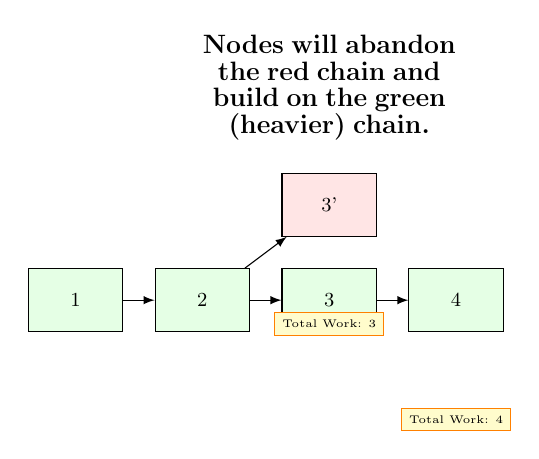
\begin{tikzpicture}[scale=0.8, every node/.style={transform shape},
    block/.style={draw, minimum width=1.5cm, minimum height=1cm, font=\small},
    work/.style={font=\tiny, fill=yellow!20, draw=orange, below, yshift=-0.2cm}
]
    % Main Chain
    \node[block, fill=green!10] (b1) {1};
    \node[block, fill=green!10, right=0.5cm of b1] (b2) {2};
    \node[block, fill=green!10, right=0.5cm of b2] (b3) {3};
    \node[block, fill=green!10, right=0.5cm of b3] (b4) {4};
    \node[work, below=of b4] {Total Work: 4};
    
    % Fork
    \node[block, fill=red!10, above=0.5cm of b3] (f1) {3'};
    \node[work, below=of f1] {Total Work: 3};

    % Arrows
    \draw[-latex] (b1) -- (b2);
    \draw[-latex] (b2) -- (b3);
    \draw[-latex] (b3) -- (b4);
    \draw[-latex] (b2) -- (f1);
    
    % Repositioned label to avoid overlap
    \node[above=0.4cm of f1, text width=5cm, align=center] (label) {\large\bfseries Nodes will abandon the red chain and build on the green (heavier) chain.};
\end{tikzpicture}
\end{center}
\vfill
\end{frame}

% ========== SLIDE 12: Implication: Probabilistic Finality ==========
\begin{frame}{Implication: Probabilistic Finality}

{\small Because a heavier chain could always emerge, a transaction's finality is never absolute—it is \textit{probabilistic}. The probability of a reorg reversing your transaction decreases as more blocks are built on top of it.}

\vfill

% Restructured layout to place diagram and key term box side-by-side
\begin{columns}[T, totalwidth=\textwidth]
    % Column for the TikZ Diagram
    \begin{column}{0.6\linewidth}
        \begin{tikzpicture}[scale=0.65, every node/.style={transform shape},
            block/.style={draw, minimum size=1.2cm, font=\small, fill=blue!10},
            txblock/.style={block, fill=armygold!50}
        ]
            \begin{scope}[start chain=going right, node distance=0.1mm]
                \node[on chain, block] (b1) {...};
                \node[on chain, txblock] (tx) {TX};
                \node[on chain, block] (k1) {k=1};
                \node[on chain, block] (k2) {k=2};
                \node[on chain, block] (k3) {k=3};
                \node[on chain, block] (k4) {k=4};
                \node[on chain, block] (k5) {k=5};
                \node[on chain, block] (k6) {k=6};
            \end{scope}

            \draw[decorate, decoration={brace, amplitude=6pt}, yshift=-0.7cm] (k1.south west) -- (k6.south east) 
                node [midway, below, yshift=-0.3cm] {\textbf{6 Confirmations}};
                
            % Risk Meter
            \draw[->, line width=7pt, red] (tx.north) ++ (0, 0.4) -- ++(0,0.8) node[midway, right, xshift=0.2cm, black] {High Risk};
            \draw[->, line width=7pt, green] (k6.north) ++ (0, 0.4) -- ++(0,0.8) node[midway, right, xshift=0.2cm, black] {Low Risk};
        \end{tikzpicture}
    \end{column}
    
    % Column for the Key Term Box
    \begin{column}{0.4\linewidth}
        \begin{keytermbox}{Key Term: Probabilistic Finality}
        \footnotesize A state where the likelihood of a transaction being reversed decreases as it gets deeper in the blockchain, but never reaches zero. Users manage this risk by waiting for a policy-based number of confirmations ($k$).
        \end{keytermbox}
    \end{column}
\end{columns}
\end{frame}

% ========== SLIDE 13: Forks, Reorgs, and Network Dynamics ==========
\begin{frame}{Forks, Reorgs, and Network Dynamics}
    \begin{itemize}
        \item \textbf{Forks}: Short-lived forks are normal. Long or frequent forks can signal network stress or an attack like selfish mining \cite{eyal_majority_2014}.
        \item \textbf{Reorgs}: When a node discovers a heavier valid chain, it switches to that new chain.
        \item \textbf{Monitoring}: Operators watch metrics like stale block rate and propagation times to assess network health.
    \end{itemize}
    \vfill
    \placeholdergraphic{A simple dashboard mock showing three metrics: Stale Rate (gauge), Propagation Delay (histogram), and Peer Connectivity (map).}
\end{frame}

% ========== SLIDE 14: Incentives and Alignment ==========
\begin{frame}{Incentives and Alignment}
    \begin{itemize}
        \item Cryptography defines what is \textit{possible}; incentives shape what is \textit{optimal}.
        \item \textbf{Rewards} (block rewards, fees) guide participants to follow the rules.
        \item \textbf{Penalties} (e.g., "slashing" in PoS) make misbehavior costly.
        \item The goal is an economic game where honesty is the dominant strategy \cite{bano_blockchain_2017}.
    \end{itemize}
    \vfill
    \begin{tcolorbox}[enhanced, colback=red!20, colframe=red!75!black, fonttitle=\bfseries, title={Incentives Complement Guarantees}, rounded corners, drop shadow]
    \small Incentives encourage correct behavior but do not replace the need for the protocol's formal safety and liveness guarantees.
    \end{tcolorbox}
\end{frame}

% ========== SLIDE 15: Trade-offs: A Visual Summary ==========
\begin{frame}{Trade-offs: A Visual Summary}
    \placeholdergraphic{A radar chart with axes for: Decentralization, Scalability, Latency, Energy Cost, and Finality Strength.
    \begin{itemize}\footnotesize
        \item PoW polygon: High on Decentralization, low on others.
        \item BFT polygon: High on performance axes, lower on Decentralization.
        \item CFT polygon: Highest on performance, but for trusted settings only.
    \end{itemize}
    }
    \vfill
    \begin{center}\large\textbf{There is no "best" protocol, only the best fit for the requirements.}\end{center}
\end{frame}

% ========== SLIDE 16: Permissioned vs. Permissionless ==========
\begin{frame}{Permissioned vs. Permissionless}
\begin{columns}[T]
    \begin{column}{0.5\linewidth}
        \begin{tcolorbox}[enhanced, colback=d2s.fg!30, colframe=black, fonttitle=\bfseries, title={Permissioned}, rounded corners, drop shadow]
            \begin{itemize}
                \item Identities are known
                \item Requires governance
                \item Uses BFT for deterministic finality
                \item For enterprise use
            \end{itemize}
        \end{tcolorbox}
    \end{column}
    \begin{column}{0.5\linewidth}
        \begin{tcolorbox}[enhanced, colback=d2s.fg!30, colframe=black, fonttitle=\bfseries, title={Permissionless}, rounded corners, drop shadow]
            \begin{itemize}
                \item Anyone can join
                \item Economic Sybil resistance
                \item Probabilistic finality
                \item For public currencies
            \end{itemize}
        \end{tcolorbox}
    \end{column}
\end{columns}
\vfill
\begin{tcolorbox}[enhanced, colback=red!20, colframe=red!75!black, fonttitle=\bfseries, title={The Deciding Factor: Identity}, rounded corners, drop shadow]
    The ability to govern who can participate determines the appropriate consensus family.
\end{tcolorbox}
\end{frame}

% ========== SLIDE 17: Selecting a Consensus: Practical Rubric ==========
\begin{frame}{Selecting a Consensus: Practical Rubric}
    A repeatable process for choosing the right consensus model:
    \begin{enumerate}
        \item \textbf{Identity and Threat Model}: Who participates? Trusted or anonymous? Crash or Byzantine?
        \item \textbf{Finality Contract}: Is deterministic finality required? What is the cost of a reorg?
        \item \textbf{Performance Envelope}: What are the latency and throughput requirements?
        \item \textbf{Operations and Incentives}: Who runs nodes? How are upgrades governed?
    \end{enumerate}
    \vfill
    \placeholdergraphic{Decision tree: "Use Case" -> "Permissioned?" -> Yes leads to "BFT (Interbank Settlement)"; No leads to "Nakamoto/PoS (Public Payments)".}
\end{frame}

% ========== SLIDE 18: CFT Deep Dive: Paxos vs Raft ==========
\begin{frame}{CFT Deep Dive: Paxos vs Raft}
    \begin{itemize}
        \item Foundational CFT protocols for keeping a replicated log consistent.
        \item \textbf{Paxos}: The original, proven correct but famously difficult to implement.
        \item \textbf{Raft}: Designed for understandability by decomposing consensus into: Leader Election, Log Replication, and Safety.
        \item Most modern CFT systems use Raft due to its clarity.
    \end{itemize}
    \vfill
    \begin{tcolorbox}[enhanced, colback=d2s.fg!30, colframe=black, fonttitle=\bfseries, title={Shared Limitation}, rounded corners, drop shadow]
    Neither protocol is designed for Byzantine faults. They are only safe within a trusted cluster.
    \end{tcolorbox}
\end{frame}


% ========== SLIDE 19: PBFT Phases and View Change ==========
\begin{frame}{PBFT Phases and View Change}
    \begin{columns}[T]
        \begin{column}{0.5\linewidth}
            \begin{tcolorbox}[enhanced, colback=d2s.fg!30, colframe=black, fonttitle=\bfseries, title={Normal Case Operation \cite{castro_practical_1999}}, rounded corners, drop shadow]
            A multi-phase process to ensure agreement:
            \begin{enumerate}
                \item \textbf{Pre-Prepare}: Leader proposes.
                \item \textbf{Prepare}: Replicas broadcast agreement.
                \item \textbf{Commit}: Replicas see a quorum and broadcast a commit.
            \end{enumerate}
            An operation is final after a quorum of commits.
            \end{tcolorbox}
        \end{column}
        \begin{column}{0.5\linewidth}
            \begin{tcolorbox}[enhanced, colback=d2s.fg!30, colframe=black, fonttitle=\bfseries, title={View Change (Failure Case)}, rounded corners, drop shadow]
            \begin{itemize}
                \item Replicas timeout if the leader stalls.
                \item They initiate a \textbf{view change} to elect a new leader.
                \item Quorum certificates are carried forward to preserve safety.
            \end{itemize}
            \end{tcolorbox}
        \end{column}
    \end{columns}
\end{frame}

% ========== SLIDE 20: Weak-Coordinator BFT Specifics ==========
\begin{frame}{Weak-Coordinator BFT Specifics}
    \begin{itemize}
        \item A modern BFT optimization for better performance in WANs.
        \item \textbf{The Rule}: Replicas follow "highest QC wins," only voting for proposals that extend the chain with the highest known Quorum Certificate.
        \item \textbf{The Coordinator's Role}: An optimizer, not a gatekeeper. Proposes blocks to speed up agreement, but is not required for progress.
        \item \textbf{The Result}: Reduced sensitivity to slow leaders and better tail latency, while preserving all BFT safety guarantees.
    \end{itemize}
\end{frame}

% ========== SLIDE 21: PoW Assumptions and Attack Surfaces ==========
\begin{frame}{PoW Assumptions and Attack Surfaces}
    \begin{tcolorbox}[enhanced, colback=d2s.fg!30, colframe=black, fonttitle=\bfseries, title={Core Assumptions for PoW Security}, rounded corners, drop shadow]
        \begin{enumerate}
            \item \textbf{Honest Majority}: An attacker controls $<50\%$ of network hash power.
            \item \textbf{Timely Propagation}: Blocks propagate quickly, so most miners work on the same tip.
        \end{enumerate}
    \end{tcolorbox}
    \begin{tcolorbox}[enhanced, colback=red!20, colframe=red!75!black, fonttitle=\bfseries, title={When Assumptions Weaken, Attacks Emerge}, rounded corners, drop shadow]
        \begin{itemize}
            \item \textbf{Selfish Mining}: Strategically withholding blocks to gain outsized rewards \cite{eyal_majority_2014}.
            \item \textbf{Eclipse/Partition Attacks}: Isolating nodes to feed them a false view of the chain.
        \end{itemize}
    \end{tcolorbox}
\end{frame}

% ========== SLIDE 22: Energy and Externalities ==========
\begin{frame}{Energy and Externalities}
    \begin{columns}[T]
        \begin{column}{0.5\linewidth}
            \begin{tcolorbox}[enhanced, colback=d2s.fg!30, colframe=black, fonttitle=\bfseries, title={Proof-of-Work}, rounded corners, drop shadow]
            Converts energy into Sybil resistance.
            \begin{itemize}
                \item \textbf{Pro}: Permissionless; anchored in physics.
                \item \textbf{Con}: High energy use \cite{mahajan_ais_2025}.
            \end{itemize}
            \end{tcolorbox}
        \end{column}
        \begin{column}{0.5\linewidth}
            \begin{tcolorbox}[enhanced, colback=d2s.fg!30, colframe=black, fonttitle=\bfseries, title={BFT / Proof-of-Stake}, rounded corners, drop shadow]
            Replaces energy with capital-at-risk.
            \begin{itemize}
                \item \textbf{Pro}: Energy-efficient.
                \item \textbf{Con}: Stake centralization risk; governance overhead.
            \end{itemize}
            \end{tcolorbox}
        \end{column}
    \end{columns}
    \vfill
    \begin{tcolorbox}[enhanced, colback=red!20, colframe=red!75!black, fonttitle=\bfseries, title={There Is No "Free" Security}, rounded corners, drop shadow]
    The cost of securing a network is paid in a different form—either energy (PoW) or locked capital and governance (PoS/BFT) \cite{bano_blockchain_2017}.
    \end{tcolorbox}
\end{frame}

% ========== SLIDE 23: Governance, Parameters, and Upgrades ==========
\begin{frame}{Governance, Parameters, and Upgrades}
    \begin{itemize}
        \item A protocol's guarantees depend on correctly configured parameters (committee sizes, thresholds, timeouts).
        \item Upgrade mechanisms vary by system type:
        \begin{itemize}
            \item \textbf{Permissionless}: Off-chain social consensus.
            \item \textbf{Permissioned}: Formal on-chain governance.
        \end{itemize}
    \end{itemize}
    \begin{tcolorbox}[enhanced, colback=red!20, colframe=red!75!black, fonttitle=\bfseries, title={The Meta-Point}, rounded corners, drop shadow]
    Consensus is not just an algorithm; it is an operational practice. Failures often stem from misconfiguration or poor governance.
    \end{tcolorbox}
\end{frame}

% ========== SLIDE 24: Mini Case Studies ==========
\begin{frame}{Mini Case Studies}
\begin{columns}[T]
    \begin{column}{0.5\linewidth}
        \begin{tcolorbox}[enhanced, colback=d2s.fg!30, colframe=black, fonttitle=\bfseries, title={Case A: Public Payments (Bitcoin)}, rounded corners, drop shadow]
            \begin{itemize}
                \item \textbf{Reqs}: Openness, censorship resistance.
                \item \textbf{Identity}: Anonymous.
                \item \textbf{Choice}: Nakamoto (PoW) \cite{nakamoto_bitcoin_2008}.
            \end{itemize}
        \end{tcolorbox}
    \end{column}
    \begin{column}{0.5\linewidth}
        \begin{tcolorbox}[enhanced, colback=d2s.fg!30, colframe=black, fonttitle=\bfseries, title={Case B: Interbank Settlement}, rounded corners, drop shadow]
            \begin{itemize}
                \item \textbf{Reqs}: Predictable latency, compliance.
                \item \textbf{Identity}: Known, regulated parties.
                \item \textbf{Choice}: BFT \cite{castro_practical_1999}.
            \end{itemize}
        \end{tcolorbox}
    \end{column}
\end{columns}
\vfill
\begin{center}\textbf{Different missions and trust assumptions lead to different technical choices.}\end{center}
\end{frame}


% ========== SLIDE 25: Bridge to Lecture 2: Consensus Approaches ==========
\begin{frame}{Bridge to Lecture 2: Consensus Approaches}
    You now have the analytical lens for evaluating consensus protocols. Next, we will apply this lens to the major \textbf{approaches} used in blockchains:
    \begin{itemize}
        \item The Longest-Chain Rule (Core of Nakamoto Consensus)
        \item Proof-of-Work (PoW): mechanism, incentives, and limitations.
        \item Proof-of-Stake (PoS): validator selection, slashing, and security assumptions.
        \item A contrast of open (permissionless) vs. closed (permissioned) settings.
    \end{itemize}
    \vfill
    \begin{tcolorbox}[enhanced, colback=red!20, colframe=red!75!black, fonttitle=\bfseries, title={Coming Up Next}, rounded corners, drop shadow]
    We will move from the general theory of consensus to the specific mechanics of Proof-of-Work and Proof-of-Stake.
    \end{tcolorbox}
\end{frame}

% --- REFERENCES SLIDE ---
\begin{frame}[allowframebreaks]{References}
    \bibliographystyle{plain}
    \bibliography{Blockchain} % Assumes your .bib file is named Blockchain.bib
\end{frame}

\end{document}